\section{Parallelization performance}
\label{sec:dsmc_parallelization_performance}
After the code is parallelized, the total computation time needed to perform a simulation is obviously not reduced. There are still as many collisions as before as the physical problem is identical. The idea is to do many of the calculations at the same time so that the total \textit{real} time we actually wait is reduced. Parallelizing is of course not free, as we need more logic to let the processors communicate with each other (exchanging particles and waiting for each other to finish each time step). As the number of processors increases, the total computation time \textit{per processor} is reduced, but the time spent on communication often increases. We will measure what's called \textit{parallel scalability} which indicates how efficient a program is when the number of processors is increased. There are two different kinds of scalability; weak and strong scaling
\begin{itemize}
	\item strong scaling is how the computation time changes with an increased number of processors on a fixed system size, whereas the
	\item weak scaling is how the computation time changes with an increased number of processors on a fixed system size \textit{per processor}.
\end{itemize}
\subsection{Strong scaling}
To see how the program efficiency scales with a fixed system size while increasing the number of processors is important if we want to study a specific system (a given system size and geometry, e.g. scanned from real data), but we would like to reduce the simulation run time. With a fixed system size, the total number of particles per CPU is obviously reduced while increasing the total number of processors. We define the \textit{strong scaling efficiency} $\eta_s$ as
\begin{align}
	\eta_s = \frac{t_1}{Nt_N},
\end{align}
where $t_1$ is the total run time using one processor and $t_N$ is the total run time using $N$ processors. We see that $\eta_s\in (0,1)$ since $Nt_N$ is the ideal scaling without any communication overhead. In this benchmark, we have run a geometry carved out by 10 random walkers (the algorithm is described in section \ref{sec:dsmc_random_walk_algorithm}), each starting at random positions. Each walker moves 1000 steps (voxels) with a turn probability of 0.1 on a $128\times128\times128$ voxel grid ending up with a porosity of $\phi=0.53635$. The physical system is a cube with side length $L=$\unit{1.0}{\micro\meter} with a density $\rho_n=\unit{1.0\e{25}}{\meter^{-3}}$ which gives a total of 5.3 million atoms. We choose that one DSMC particle represents one atom yielding a total of 5.3 million particles in the whole system. The benchmark was performed with $2^N$ processors from 1 CPU to 512 CPUs yielding a good estimate of how efficient the program scales for a relatively large number of processors. In table \ref{tab:dsmc_strong_scaling} we have the results with additional information like the CPU configuration $(P_x, P_y, P_z)$ as defined in section \ref{sec:dmsc_parallelization}. The strong scaling efficiency is plotted against the number of processors in figure \ref{fig:dsmc_strong_scaling}.
\begin{table}
\begin{center}
    \begin{tabular}{|l|l|l|l|l|l}
    \hline
    $N_\text{CPU}$ & $(P_x, P_y, P_z)$ & $N_\text{particles}/N_\text{CPU}$ & Run time[s] & $\eta_s$ \\ \hline
    1 & (1,1,1) & 5.4\e{6} & \unit{10571}{\second} & 1.00\\
    \hline
    2 & (1,1,2) & 2.7\e{6} & \unit{5262}{\second} & 1.00\\
    \hline
    4 & (1,2,2) & 1.3\e{6} & \unit{2687}{\second} & 0.984\\
    \hline
    8 & (2,2,2) & 6.7\e{5} & \unit{1360}{\second} & 0.972\\
    \hline
    16 & (2,2,4) & 3.4\e{5} & \unit{755}{\second} & 0.875\\
    \hline
    32 & (2,4,4) & 1.7\e{5} & \unit{505}{\second} & 0.654\\
    \hline
    64 & (4,4,4) & 8.4\e{4} & \unit{262}{\second} & 0.630\\
    \hline
    128 & (4,4,8) & 4.2\e{4} & \unit{146}{\second} & 0.566\\
    \hline
    256 & (4,8,8) & 2.1\e{4} & \unit{94}{\second} & 0.440\\
    \hline
    512 & (8,8,8) & 1.0\e{4} & \unit{79}{\second} & 0.261\\
    \hline
    \end{tabular}
    \caption{Benchmark results showing the strong scaling efficiency $\eta_s$ for the DSMC program.}
    \label{tab:dsmc_strong_scaling}
    \end{center}
\end{table}

\begin{figure}[h]
\begin{center}
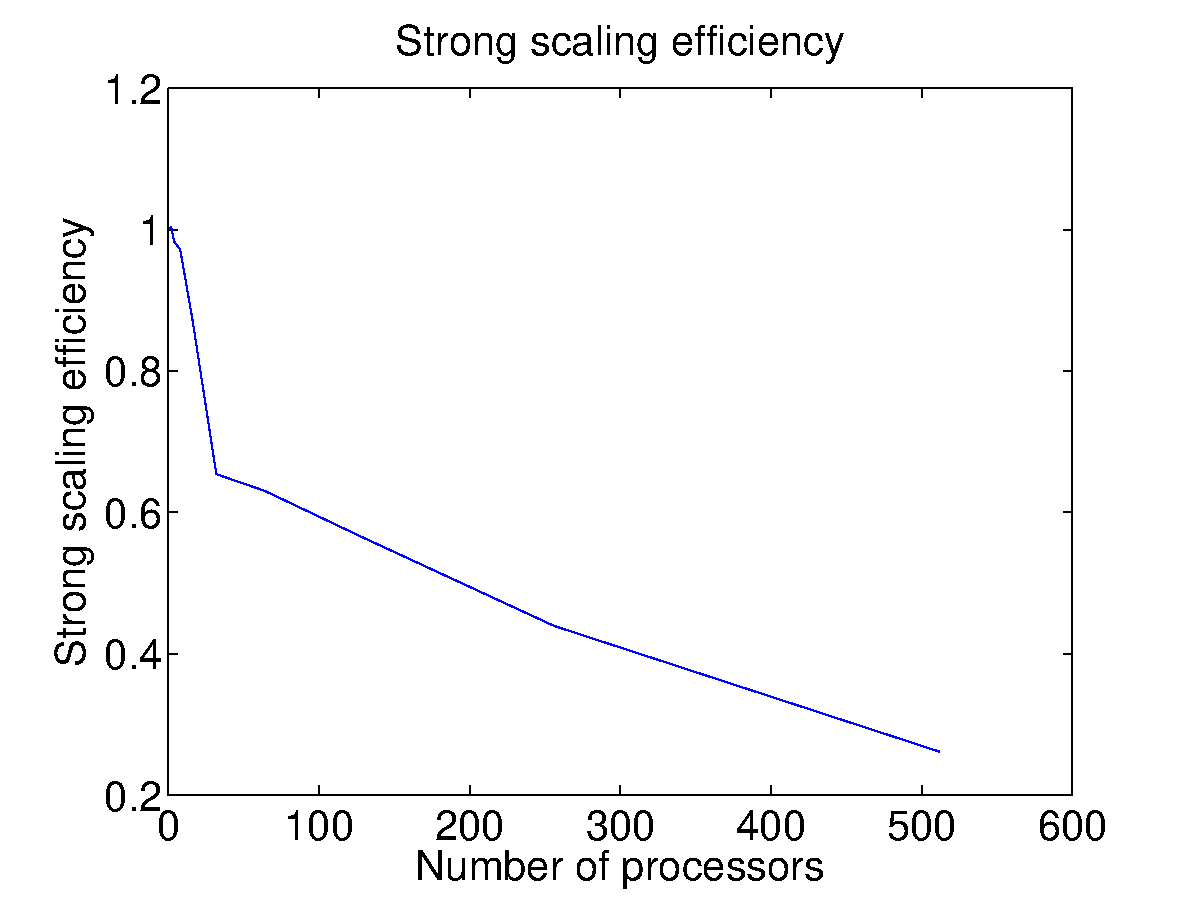
\includegraphics[width=\textwidth, trim=0cm 0cm 0cm 0cm, clip]{DSMC/figures/strong_scaling.eps}
\end{center}
\caption{The strong scaling efficiency $\eta_s$ as a funtion of the number of processors $N_\text{CPU}$. We see that at 512 processors, the efficiency is reduced to 25\% because of the large overhead from the MPI communication.}
\label{fig:dsmc_strong_scaling}
\end{figure}
The reason for this scaling behavior might be due to bad load balancing since the processors might get different work load. One processor might get a subvolume that contains very few particles if most of its voxels are solid wall voxels. These processors will spend most of their time on waiting for the other processors to finish and we do not make full use of the available processors. This problem is discussed further in section \ref{sec:future_work_load_balancing}. 
\subsection{Weak scaling}
Another important scaling problem appears when we want to maximize the simulated system size. If we keep a constant system size \textit{per cpu}, and increase the number of processors, the limitation of how big we efficiently can create the system is controlled by the weak scaling. We then introduce the \textit{weak scaling efficiency} $\eta_w$ defined as
\begin{align}
	\eta_w = \frac{t_1}{t_N},
\end{align}
where again $t_1$ is the total run time using one processor and $t_N$ is the run time using $N$ processors. If the algorithm scales perfectly, the total run time would remain constant while increasing the number of processors (each CPU is ideally independent), but we expect some overhead. This implies that the range for $\eta_w$ also is between zero and one. We have run the same geometry as for the strong scaling, but each processor controls a volume of \unit{1}{\micro\meter^3} so that the largest system is \unit{512}{\micro\meter^3}. Keeping the same density gives a total of 5.3 million particles per processor. In table \ref{tab:dsmc_weak_scaling}, we have the results for the weak scaling efficiency simulation. 
\begin{table}
\begin{center}
    \begin{tabular}{|l|l|l|l|l|l}
    \hline
    $N_\text{CPU}$ & $(P_x, P_y, P_z)$ & $N_\text{particles}$ & Run time[s] & $\eta_w$ \\ 
    \hline
    1 & (1,1,1) & 5.4\e{6} & \unit{100}{\second} & 1.0\\
    \hline
    2 & (1,1,2) & 1.27\e{6} & \unit{100}{\second} & 1.0\\
    \hline
    4 & (1,2,2) & 1.27\e{6} & \unit{100}{\second} & 1.0\\
    \hline
    8 & (2,2,2) & 1.27\e{6} & \unit{100}{\second} & 1.0\\
    \hline
    16 & (2,2,4) & 1.27\e{6} & \unit{100}{\second} & 1.0\\
    \hline
    32 & (2,4,4) & 1.27\e{6} & \unit{100}{\second} & 1.0\\
    \hline
    64 & (4,4,4) & 1.27\e{6} & \unit{100}{\second} & 1.0\\
    \hline
    128 & (4,4,8) & 1.27\e{6} & \unit{100}{\second} & 1.0\\
    \hline
    256 & (4,8,8) & 1.27\e{6} & \unit{100}{\second} & 1.0\\
    \hline
    512 & (8,8,8) & 1.27\e{6} & \unit{100}{\second} & 1.0\\
    \hline
    \end{tabular}
    \caption{Benchmark results showing the weak scaling efficiency $\eta_w$ for the DSMC program.}
    \label{tab:dsmc_weak_scaling}
    \end{center}
\end{table}
\section{Results for simple geometries}
\label{sec:results_for_simple_geometries}
In this section, we will study flow in simple geometries where the theoretical permeability is well known. The expression for the permeability is only valid for small Knudsen numbers (which we called the absolute permeability; the permeability for fluids in the continuum limit), so it is a perfect test case for the Knudsen correction factor $f_c$ in equation \eqref{eq:knudsen_correction}. 

\subsection{Flow in a cylinder, varying Knudsen number}
We have induced flow in a cylinder with radius \unit{0.45}{\micro\meter} with an applied acceleration corresponding to a pressure difference $\Delta P = 1.1P_0$, where $P_0$ is the ideal gas pressure at \unit{300}{\kelvin}. We want to vary the Knudsen number which was defined as
\begin{align}
	\text{Kn} = \frac{\lambda}{L} = \frac{1}{\sqrt 2 \pi d^2 \rho_n L}
\end{align}
where $L$ is the length of the cylinder, $\lambda$ is the mean free path. We have used equation \eqref{eq:mean_free_path} in the last expression so that we can choose the Knudsen number through the density
\begin{align}
	\rho_n(\text{Kn}) = \frac{1}{\sqrt 2 \pi d^2 \text{Kn}L}.
\end{align}
We expect an apparent permeability satisfying the Knudsen correction
\begin{align}
	k_a = k_\infty f_c = k_\infty[1 + \alpha(\text{Kn})\text{Kn}]\left[1 + {4\text{Kn}\over 1 + \text{Kn}}\right].
\end{align}
The analytical absolute permeability for a cylinder with radius $r$ is given by\cite{karniadakis2005microflows}
\begin{align}
	\label{eq:permeability_cylinder}
	k_\infty = {r^2\over 8},
\end{align}
which gives the following prediction for the apparent permeability
\begin{align}
	k_a = [1 + \alpha(\text{Kn})\text{Kn}]\left[1 + {4\text{Kn}\over 1 + \text{Kn}}\right] {r^2\over 8}.
\end{align}
In figure \ref{fig:one_cylinder_varying_knudsen} we have plotted the measured permeability as a function of Knudsen number. We see that the 

\begin{figure}[h]
\begin{center}
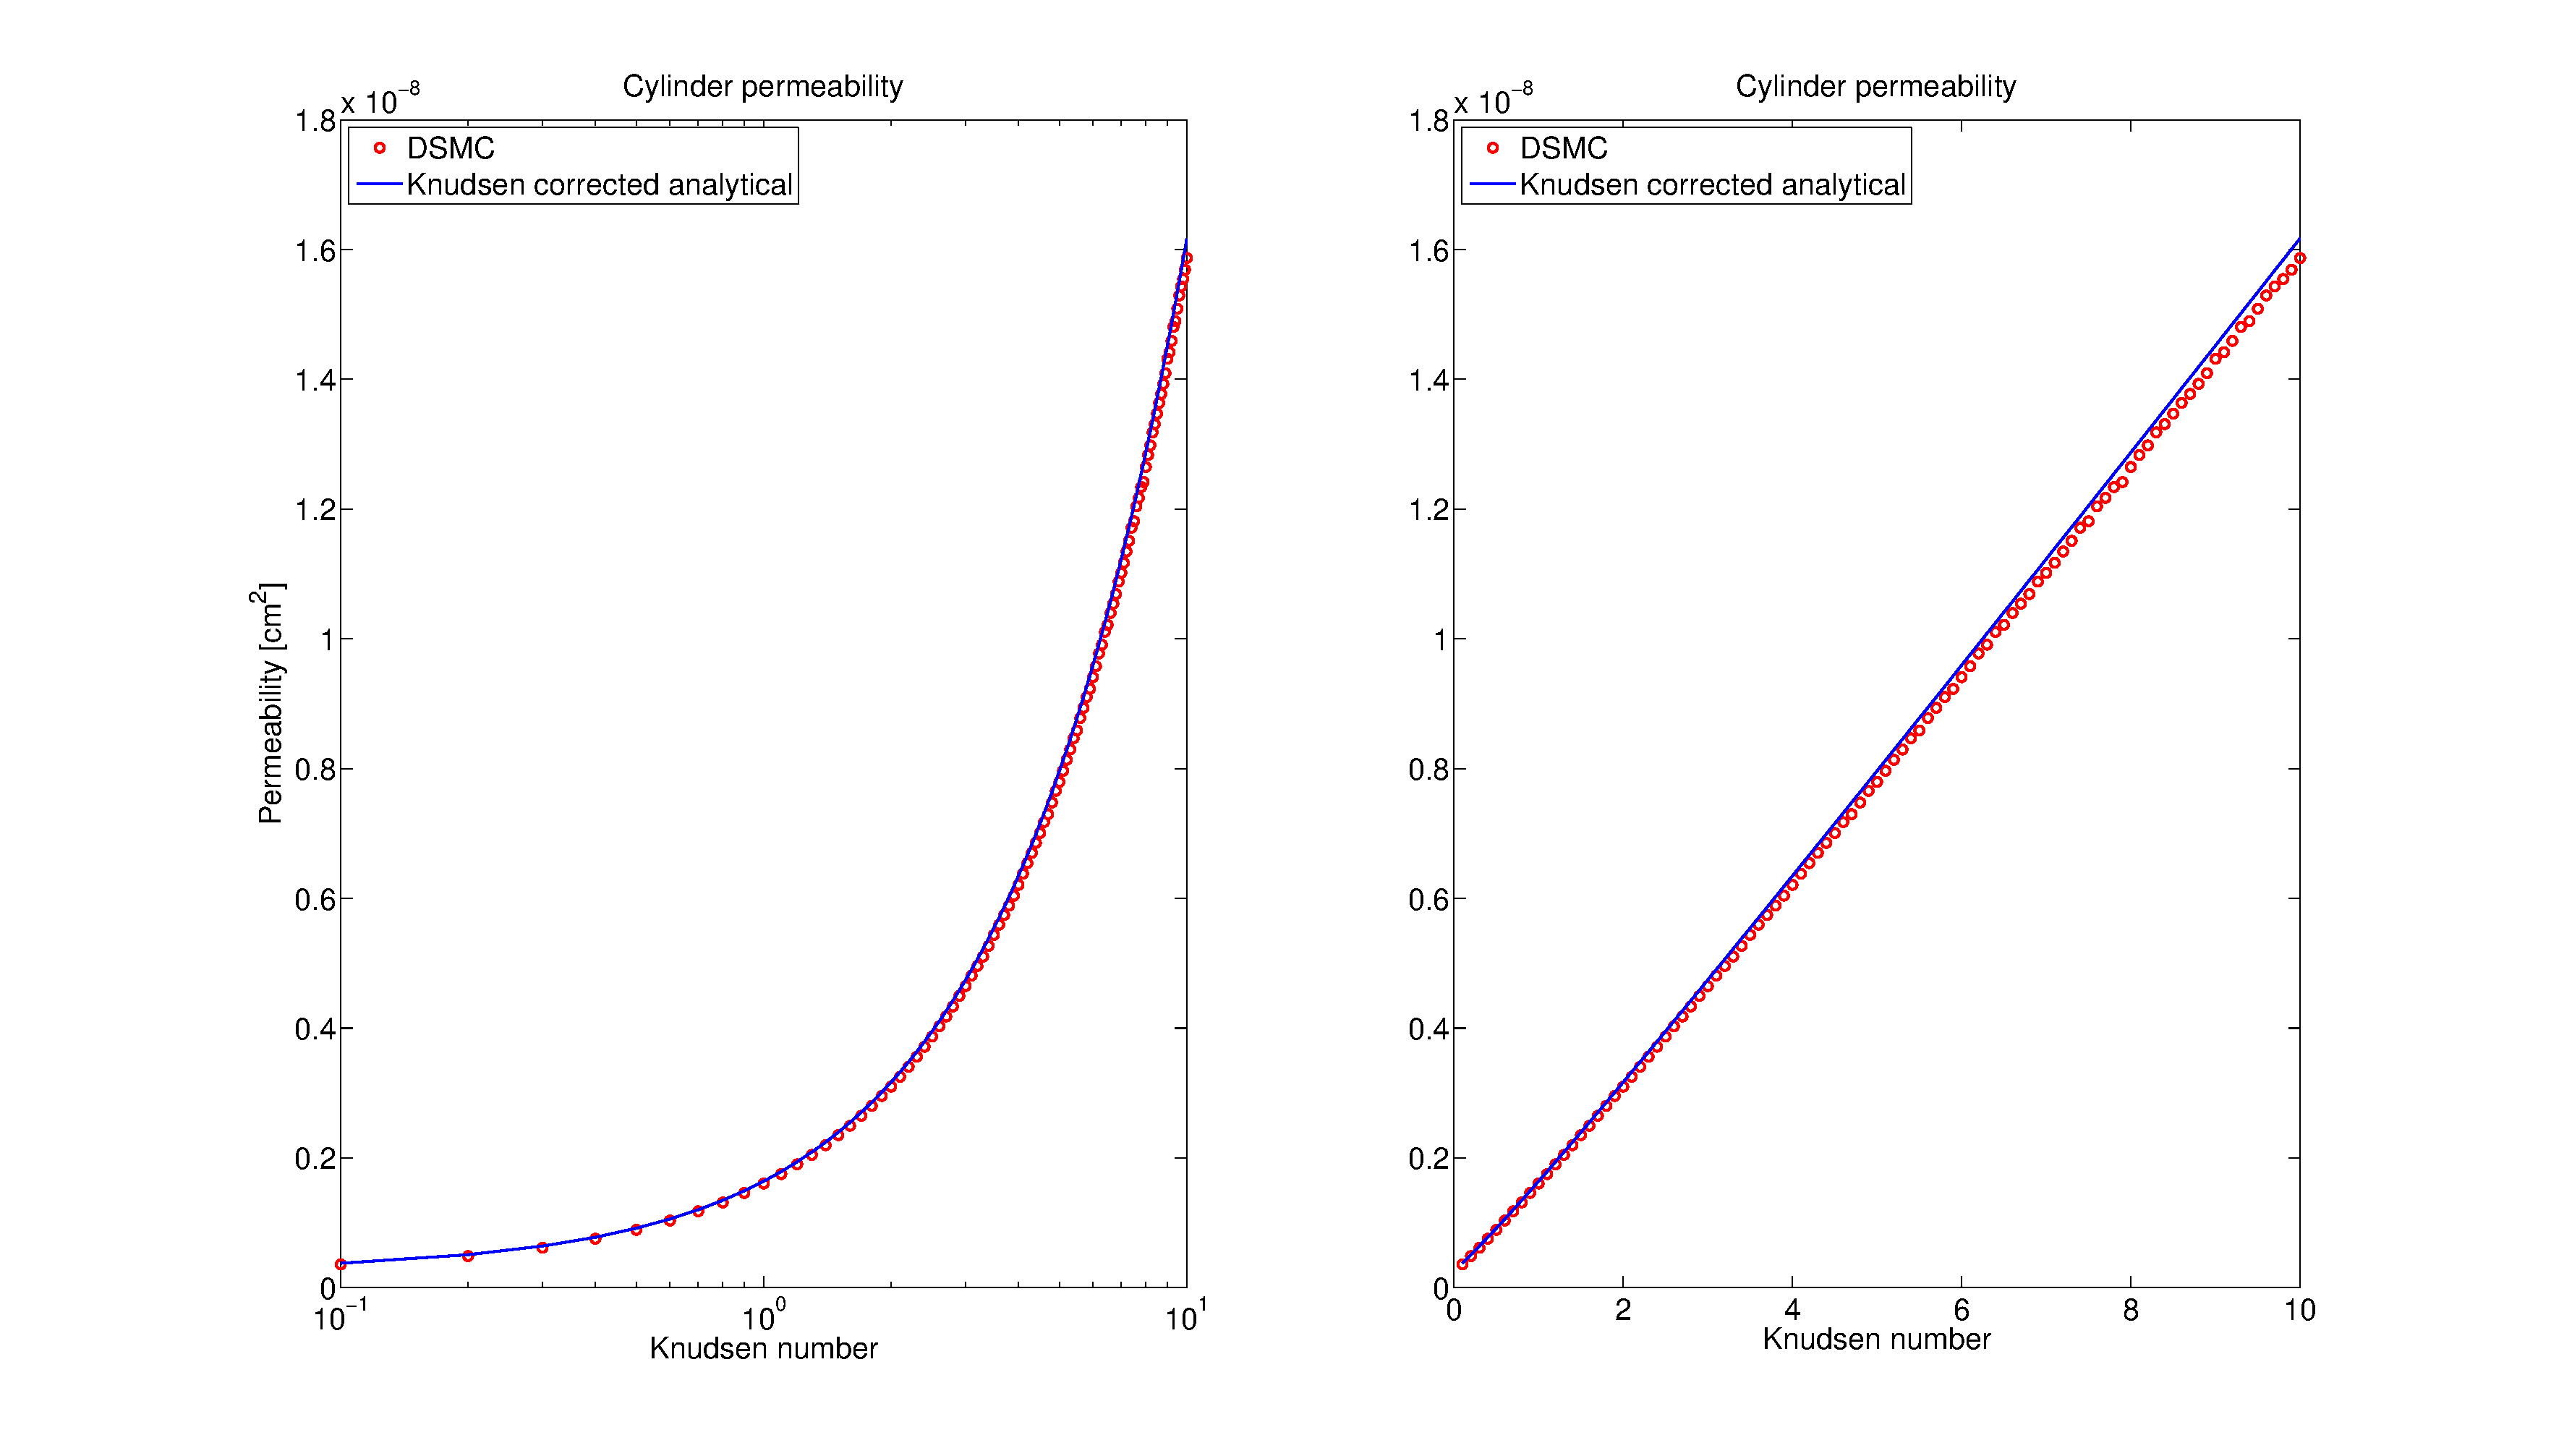
\includegraphics[width=\textwidth, trim=0cm 0cm 0cm 0cm, clip]{DSMC/figures/cylinder_knudsen_permeability.eps}
\end{center}
\caption{Permeability as a function of Knudsen number for a cylinder with radius \unit{0.45}{\micro\meter} and length \unit{1}{\micro\meter} with an applied pressure difference $\Delta P = 1.1P_0$ ($P_0$ being the ideal gas pressure). We control the Knudsen number by varying the density. The blue line is the Knudsen corrected analytical solution from \cite{karniadakis2005microflows}. The DSMC results confirm that the Knudsen correction factor works very well for a system with a well defined Knudsen number.}
\label{fig:one_cylinder_varying_knudsen}
\end{figure}

\subsection{Flow in a cylinder, varying radius}
If we instead keep the Knudsen number constant ($\text{Kn}=1.0$), we can vary the radius to verify equation \eqref{eq:permeability_cylinder}. We have studied radii in the range \unit{0.1}{\micro\meter} to \unit{0.45}{\micro\meter} with the same pressure difference as in the previous simulation ($\Delta P = 1.1P_0)$. In figure \ref{fig:one_cylinder_varying_radii_result} we have plotted the measured permeability as a function of cylinder radius. The straight line confirms the quadratic dependency in equation \eqref{eq:permeability_cylinder}.
\begin{figure}[h]
\begin{center}
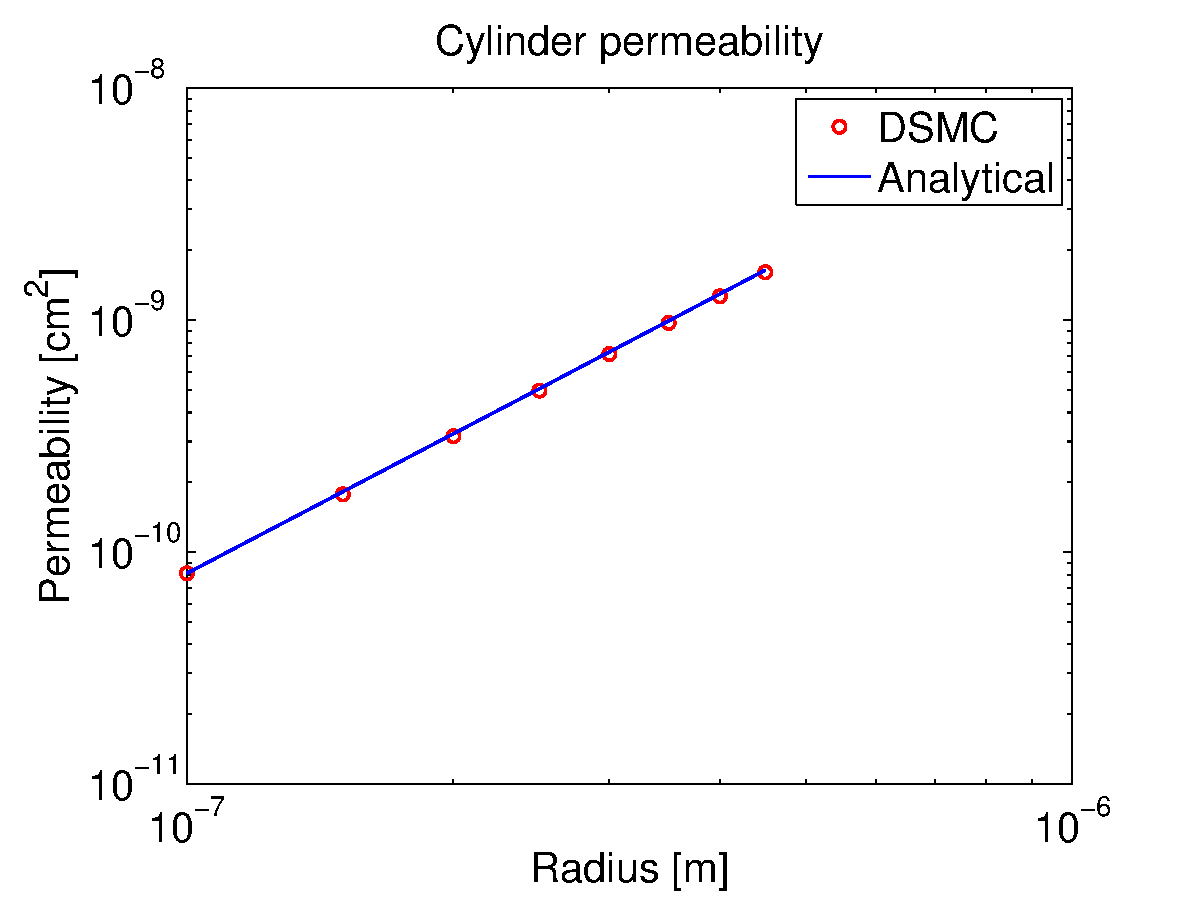
\includegraphics[width=\textwidth, trim=0cm 0cm 0cm 0cm, clip]{DSMC/figures/cylinder_radius_permeability.eps}
\end{center}
\caption{Logarithmic plot of the permeability for different cylinders with radii in the range $0.1 \mu m$ to $0.45 \mu m$ with an applied pressure difference $\Delta P = 1.1P_0$. The blue line is the Knudsen corrected analytical solution from \cite{karniadakis2005microflows}.}
\label{fig:one_cylinder_varying_radii_result}
\end{figure}
\section{Results for complicated geometries}
\subsection{Randomly packed spheres}
Through the Carman-Kozeny equation, we can theoretically predict the permeability for randomly packed spheres 
\begin{align}
	k = {a^2 \over 9K} {\phi^3 \over (1 - \phi)^2},
\end{align}
where $\phi$ is the porosity, $a$ is the sphere radius and $K$ is the Kozeny constant which is experimentally measured to be around five\cite{carman1937fluid}. This theoretical result has been verified to predict permeabilities in experiments. At micrometer scale however, we expect deviations due to the high Knudsen number. 
